\clearpage
\section{Konzept}\label{sec:Konzept}
Der Aufbau des digitalen Theremin ist sehr ähnlich wie das des analogen, mit einigen Änderungen um es besser digital Aufzubauen. Abbildung \ref{img:Blockschaltbild_digital} zeigt, dass der Lautstärke- und Tonhöhenoszillator neu nicht mehr einen Sinus sondern einen Rechteck generieren. Wir haben uns deshalb für diese Änderung entschieden, da es so einfacher ist das Signal in das FPGA einzulesen, da kein Analog-Digital-Wandler nötig ist. Da der Referenzoszillator weiterhin ein Sinus ist, ergibt die Mischung mit dem Rechteck, welcher Oberwellen hat, neu auch Mischprodukte mit diesen Oberwellen. Da diese aber eine höhere Frequenz haben, können diese später weggefiltert werden.\\
Weiter sind die Referenzoszillatoren neu digital. Um nun einen Sinus zu generieren, haben wir uns entschieden den in Kapitel \ref{subsec:Cordic} behandelten Cordic Algorithmus zu verwenden. Dieser ist besser um verschiedene Frequenzen zu generieren als eine einfache Lookup-Table und bietet einen grösseren Lerngewinn. Diese Komponente stammt aus dem Projekt 5. \\
Der Mischer multipliziert die beiden Signale des Referenzoszillators und analogen Oszillators.\\
Für das Tiefpassfilter haben wir uns entschieden mehrere CIC-Filter und ein FIR-Filter einzusetzten. Das CIC-Filter stammt ebenfalls aus dem Projekt 5. CIC-Filter haben den Vorteil, dass sie Ressourcensparender sind als äquivalente FIR-Filter.\\
Wie man sieht ist die Signalverarbeitung für den Lautstärketeil anders als bei der analogen Variante hier gleich wie der Tonhöhen Teil.

\begin{figure}[h]
	\centering
	\includegraphics[width=\textwidth]{Blockschaltbild_digital.pdf}
	\caption{Blockschaltbild des digitalen Theremins}
	\label{img:Blockschaltbild_digital}
\end{figure}